\documentclass[a4paper,11pt]{article}
\usepackage{polski}
\usepackage[utf8]{inputenc}
\usepackage{enumerate}
\usepackage{amssymb}		% pakiet do symboli
\usepackage{amsmath}		% pakiet do matmy
\usepackage{enumitem}		% punktowanie (a), (b), ...
\usepackage{graphicx}		% wstawianie obrazkow
\usepackage{float}			% wstawianie obrazkow w dowolnym miejscu
\usepackage{tabstackengine} 	% macierze
\usepackage{fancyhdr}		% ładniejszy wygląd stronki
\usepackage{color}   		% kolorowanie linków / odnośników
\usepackage{hyperref}
\hypersetup{
    colorlinks=true, 	% set true if you want colored links
    linktoc=all,     	% set to all if you want both sections and subsections linked
    linkcolor=black,  	% choose some color if you want links to stand out
}
\usepackage{titling}

\stackMath

% nowe komendy dla wygodniejszego pisania :)
\newcommand{\subtitle}[1]{ \posttitle{ \par\end{center} \begin{center}\large#1\end{center} \vskip0.5em}}
\newcommand{\floor}[1]{\left\lfloor #1 \right\rfloor}
\newcommand{\ceil}[1]{\left\lceil #1 \right\rceil}

% Wyglad strony:
\pagestyle{fancy}
\fancyhf{}
\chead{\leftmark}
\cfoot{\thepage}

\author{Tomasz Woszczyński}
\title{Analiza numeryczna w pigułce}
\subtitle{Definicje, wzory, twierdzenia \\ Podsumowanie informacji z semestru zimowego 2019/2020}
\date{}

\begin{document}
\thispagestyle{empty}
\maketitle
\thispagestyle{empty}

\newpage
\thispagestyle{empty}
\mbox{}
\newpage

\newpage
\setcounter{page}{1}
\tableofcontents

\clearpage
\section{Teoria błędu}
\subsection{Błąd względny i bezwzględny}
Niech $x$ będzie dokładną wartością, a $\bar{x}$ wartością przybliżoną. Błąd bezwzględny ma wartość $\left| x-\bar{x} \right|$, a błąd względny $\left| \frac{x-\bar{x}}{x} \right|$.
\subsection{Reprezentacja liczb}
\begin{enumerate}[label=(\alph*)]
\item Całkowite: $l\in\mathbb{Z} \Rightarrow l=\pm\sum\limits_{i=0}^{n} e_{i}2^{i}$, gdzie $e_i \in \{0, 1\}, e_n = 1$.
\item Rzeczywiste: $x\in\mathbb{R} \Rightarrow x=s \cdot m \cdot 2^{c}$, gdzie $s\in\{1, -1\}$ (znak), \\
$m \in \left[\frac{1}{2}, 1\right)$ (mantysa), $c \in \mathbb{Z}$ (cecha).
\end{enumerate}

\subsection {Rodzaje zaokrągleń}
Rozwinięcie dwójkowe liczb rzeczywistych jest zwykle nieskończone, dlatego używamy dwóch typów zaokrągleń:
\begin{enumerate}[label=(\alph*)]
\item Obcięcie: $m \approx m_{t}^{c} := \sum\limits_{i=1}^{t} e_{-i}\cdot 2^{-i}$, tzn. ignorujemy cyfry od $t+1$.
\item Zaokrąglenie symetryczne: $m \approx m_{t}^{r} := \sum\limits_{i=1}^{t} e_{-i}\cdot 2^{-i}+e_{-(t+1)}\cdot 2^{-t}$.
\end{enumerate}
Reprezentację zmiennopozycyjną liczby $x = s\cdot m \cdot 2^{c} \in \mathbb{R}$ nazywamy liczbę:
\begin{itemize}
\item $chop(x) := s\cdot m_{t}^{c} \cdot 2^{c}$ (obcięcie - chopping)
\item $rd(x) :=s\cdot m_{t}^{r} \cdot 2^{c}$ (zaokrąglenie symetryczne - symmetric rounding)
\end{itemize}
\textbf{Twierdzenie:}
$$ \left| \frac{x-chop(x)}{x}\right| \leq 2\cdot2^{-t} $$
$$ \left| \frac{x-rd(x)}{x} \right| \leq 2^{-t} $$

\subsection{Zbiór liczb zmiennopozycyjnych, nadmiar i niedomiar}
Weźmy $D=2^{c_{max}}$  i zdefiniujmy zbiór 
$$\mathcal{X} := \left(-D, -\frac{1}{2D}\right] \cup \{0\} \cup \left[\frac{1}{2D}, D\right)$$
Nadmiarem są wtedy wszystkie liczby ze zbioru $\left(-\infty, -D\right] \cup \left[D, \infty\right)$, a niedomiarem liczby ze zbioru $\left(-\frac{1}{2D}, \frac{1}{2D}\right) \setminus \{0\}$ - nie da się ich przedstawić w reprezentacji zmiennopozycyjnej wcześniej przez nas zdefiniowanej. Wtedy zbiorem liczb zmiennopozycyjnych nazwiemy zbiór 
$$ \mathcal{X}_{fl} := rd\left(\mathcal{X}\right)$$

\subsection{Działania arytmetyczne w świecie liczb zmiennopozycyjnych}
Weźmy $x, y \in \mathcal{X}_{fl}$ i określmy działanie $\circ \in \{+,-,\cdot, /\}$. Dla $x \circ y \in \mathcal{X}'$, czyli wyniku działania bez nadmiaru zachodzi własność
$$ fl\left(x \circ y \right) := \left( x \circ y \right)\left( 1 + \mathcal{E}_{x, y, \circ}\right) $$
gdzie $\mathcal{E}_{x, y, \circ} \leq 2^{-t}$, a $t$ to liczba bitów na zapamiętanie mantysy.
\newline Błąd względny operacji $\circ$ wynosi co najwyżej $2^{-t}$.

\subsection{Twierdzenie o kumulacji błędów}
Jeśli $\left| \delta_{i} \right| \leq 2^{-t}$, $\left( i = 1,2,\ldots, n\right)$, to zachodzi równość
$$ \prod\limits_{i=1}^{n} \left( 1 + \delta_{i} \right) = 1 + \sigma_{n} $$
dla $\sigma_{n} = \sum\limits_{i=1}^{n} \delta_{i} + O(2^{-2t})$. Jeśli $n\cdot 2^{-t} \textless 2$, to $\left| \sigma_{n} \right| \lesssim n\cdot 2^{-t}$.

\subsection{Zjawisko utraty cyfr znaczących}
Operacja $+$ liczb tych samych znaków oraz odejmowanie liczb przeciwnych znaków oraz $\cdot$ i $/$ są uznawane za "bezpieczne". Kłopot występuje wtedy, gdy odejmujemy od siebie liczby tych samych znaków. Następuje to w przypadku liczb bardzo bliskich sobie, ponieważ znormalizowanie liczby "obcina" początkowe zera w liczbie $x-y$, jednak wtedy ostatnie niezerowe cyfry są przesuwane na pierwsze pozycje i jeżeli $i\textless t$, to nie będzie wiadomo czym zapełnić pozostałe miejsca w mantysie.


\clearpage
\section{Uwarunkowanie zadania, numeryczna poprawność}
\subsection{Zadanie źle uwarunkowane i dobrze uwarunkowane}
Zadania, w których mała względna zmiana danych powoduje dużą względną zmianę wyniku nazywamy zadaniami źle uwarunkowanymi. Wielkości mówiące o tym w jaki sposób względna zmiana danych wpływa na względną wartość wyniku nazywamy wskaźnikami uwarunkowania. Zadania, które nie są źle uwarunkowane nazywamy zadaniami dobrze uwarunkowanymi.

\subsection{Wskaźnik uwarunkowania zadania}
Wzorem ogólnym jest
$$Cond(x) := \frac{\text{względna zmiana wyniku}}{\text{względna zmiana danych}}$$
Wzór ten można łatwo sprawdzić na przykładzie, wyprowadzając wskaźnik uwarunkowania zadania obliczania wartości funkcji $f$ w punkcie $x$. Względna zmiana danych wyrażana jest przez $\left| \frac{(x+\delta)-x}{x}\right| = \left| \frac{\delta}{x} \right|$, a względna zmiana wyniku przez $\left| \frac{f(x+\delta)-f(x)}{f(x)}\right|$. Po podstawieniu tych wartości do powyższego wzoru (i zauważenie, że po rozpisaniu jeden wyraz zamienia się na pochodną funkcji $f$ w punkcie $x$) otrzymujemy wzór na wskaźnik uwarunkowania zadania:
$$ Cond(x) = \left| \frac{x\cdot f'(x)}{f(x)} \right|$$

\subsection{Algorytm numerycznie poprawny}
Algorytm nazywamy numerycznie poprawnym, jeśli wynik jego działania w świecie liczb zmiennopozycyjnych może być zinterpretowany jako mało zaburzony wynik dokładny dla mało zaburzonych danych. Chcąc wyznaczyć wartość $A(a)$ w świecie liczb zmiennopozycyjnych otrzymamy
$$fl(A(a)) = (A(a\cdot(1+\beta)))\cdot(1+\alpha)$$
gdzie $(1+\beta)$ oznacza małe zaburzenie danych, a $(1+\alpha)$ małe zaburzenie wyniku.


\clearpage
\section{Rozwiązywanie równań nieliniowych}
Naszym zadaniem jest znalezienie miejsca zerowego funkcji $f \in C[a,b]$ spełniającej warunki $f(a)f(b) \textless 0$ oraz $!\exists \alpha \in [a,b] \ \ f(\alpha)=0$.

\subsection{Metoda bisekcji}
Metoda ta polega na rekurencyjnym wyznaczaniu środka przedziału, a następnie sprawdzaniu czy miejsce zerowe znajduje się po lewej czy prawej stronie i przejściu na odpowiednią z nich. Ten rekurencyjny krok powtarzamy do momentu osiągnięcia odpowiedniego przybliżenia lub dokładnie miejsca zerowego.

\begin{figure}[H]
\centering
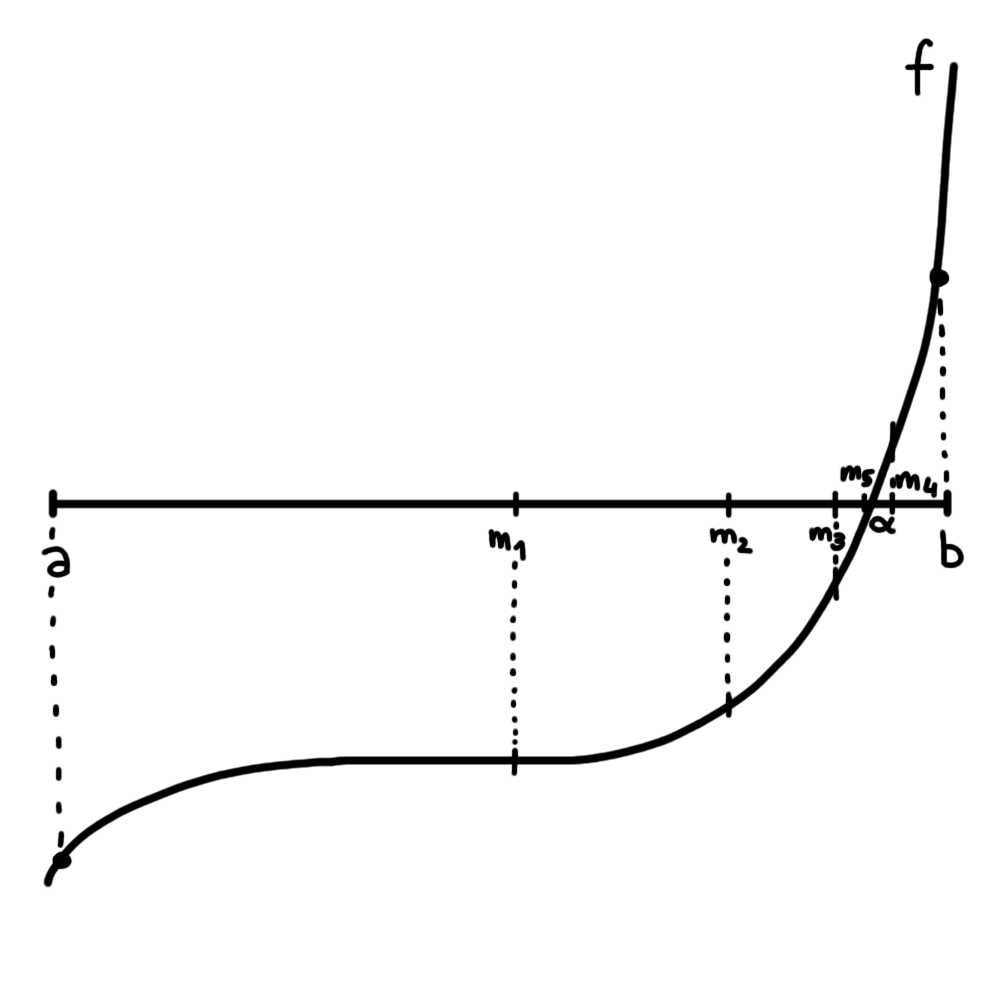
\includegraphics[width=0.66\textwidth]{metodabisekcji.png}
\caption{Przykład działania metody bisekcji}
\label{metodabisekcji}
\end{figure}

\noindent Niech $I_k := [a_k, b_k]$ dla $k=0,1,\ldots$ takie, że $I_0 \textgreater I_1 \textgreater \ldots \textgreater I_k \textgreater \ldots$ i $\alpha \in I_k$. Wyznaczmy środek k-tego przedziału jako $m_{k+1}=\frac{a_k+b_k}{2}$. Jeśli $f(m_{k+1})=0$, to $\alpha=m_{k+1}$, w przeciwnym wypadku naszym nowym przedziałem staje się $[a_k, m_{k+1}]$, gdy $f(m_{k+1}) \textgreater 0$ lub $[m_{k+1}, b_k]$, gdy $f(m_{k+1}) \textless 0$. 
\newline Metodę tę cechują:
\begin{itemize}
\item długość k-tego przedziału wynosi $|I_k|=\frac{b_0-a_0}{2^k}$ dla $k\in\mathbb{N}$.,
\item $|\alpha-m_{k+1}| \leq \frac{b_0-a_0}{2^{k+1}}$
\item wyznaczenie przybliżenia $m_{k+1}$ z błędem bezwzględnym na poziomie danego $\mathcal{E}$ przebiega w $\ceil{\log_{2}\left( \frac{b_0-a_0}{2\mathcal{E}} \right) }$ krokach
\end{itemize}

\subsection{Metoda Newtona (metoda stycznych)}
Metoda Newtona polega na wybraniu punktu $x_0$, a następnie rekurencyjne wyznaczanie kolejnych punktów kontrolnych
$$ x_{n+1} := x_n - \frac{f(x_n)}{f'(x_n)} \text{ dla } (n=0,1,2,\ldots) $$

\begin{figure}[H]
\centering
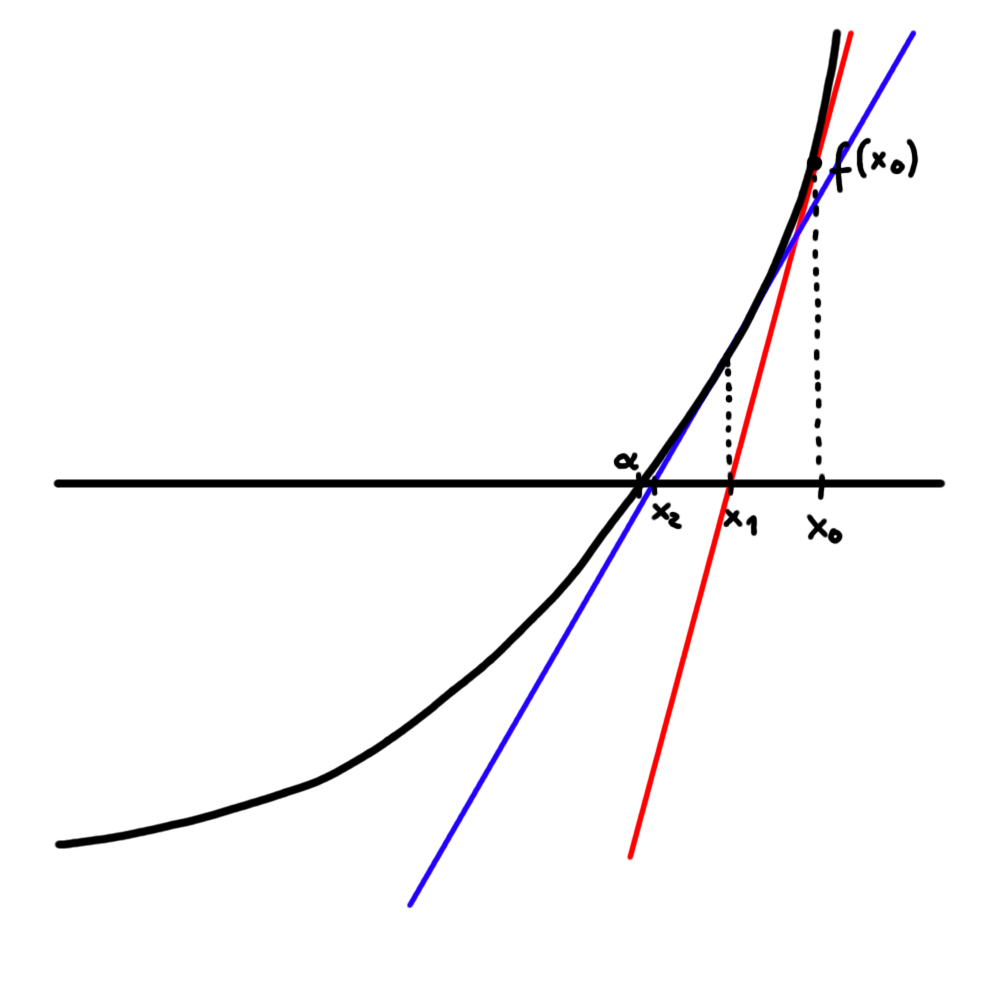
\includegraphics[width=0.66\textwidth]{metodastycznych.png}
\caption{Przykład działania metody Newtona (stycznych)}
\label{metodastycznych}
\end{figure}

Metodę tę cechują:
\begin{itemize}
\item dobry wybór $x_0$ skutkuje szybką zbieżnością do miejsca zerowego $\alpha$
\item konieczność znajomości pochodnej $f'$, co w przypadku złożonych funkcji jest problematyczne
\item czułość na dobór $x_0$ (dla $f(x)=\arctan(x-1)-\frac{1}{x^2+1}$ i $x_0=2.3604$ po 13-tej iteracji osiągamy 18-cyfrową dokładność, lecz dla $x_0=2.3605$ ciąg $x_n$ dąży do nieskończoności)
\item możliwość zapętlenia się (gdy $x_n = x_{n+1}$)
\item warunkiem stopu jest osiągnięcie $|f(x_n)| < \delta$ oraz
$$ \left| \frac{x_{n+1}-x_{n}}{x_{n}} \right|, \left| \frac{x_{n+2}-x_{n+1}}{x_{n+1}} \right|, \ldots, \left| \frac{x_{n+k}-x_{n+k-1}}{x_{n+k-1}} \right| \textless \ \mathcal{E} \text{ dla } k=2,3,\ldots $$
lub $n \geq N_{max}$ (przekroczenie limitu wywołań)
\end{itemize}

\subsection{Metoda siecznych}
Metoda siecznych polega na wybraniu punktów początkowych $x_0$ oraz $x_1$, a następnie przeprowadzaniu między nimi siecznej. Następnie dla powstałego na przecięciu punktu powtarzamy operację, zmieniając punkty na których pracujemy. Wzór rekurencyjny metody jest następujący:
$$ x_{n+1} := x_n - \frac{f(x_n)}{\frac{f(x_n)-f(x_{n-1})}{x_n-x_{n-1}}}$$

\begin{figure}[H]
\centering
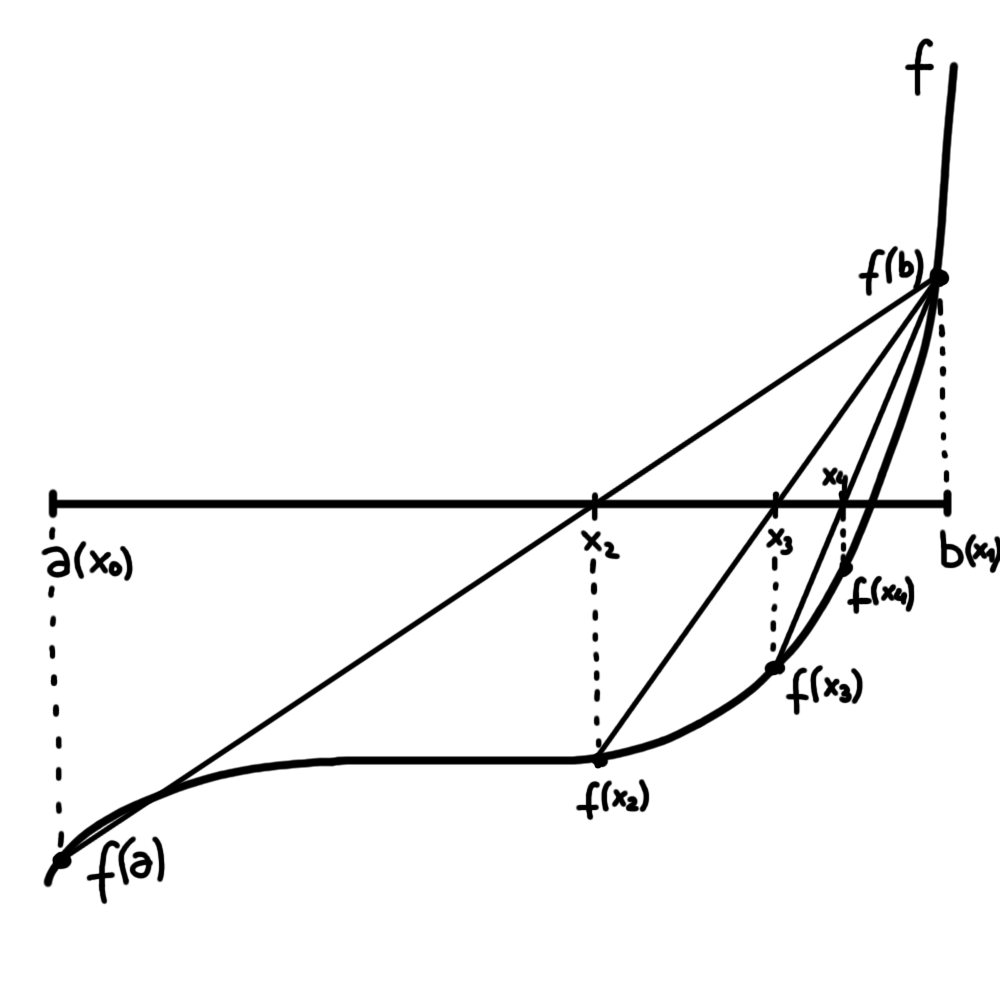
\includegraphics[width=0.66\textwidth]{metodasiecznych.png}
\caption{Przykład działania metody siecznych}
\label{metodasiecznych}
\end{figure}

Metodę tę cechują:
\begin{itemize}
\item brak konieczności obliczania pochodnej
\item wolniejszy czas działania niż przy metodzie Newtona
\item punkty startowe $x_0$ oraz $x_1$ muszą zostać intuicyjnie wybrane
\item możliwość zapętlenia się
\item duża wrażliwość na dobór $x_0$ oraz $x_1$
\item warunek stopu podobny jak w metodzie Newtona
\end{itemize}

\subsection{Wykładnik zbieżności ciągu (rząd metody)}
Niech dany będzie ciąg $(x_n)$ taki, że $\lim\limits_{n\to\infty} x_n=g$. Jeśli istnieje stałe $p$ oraz $C\in\mathbb{R}_{+}$, dla których zachodzi własność
$$ \lim\limits_{n\to\infty} \frac{\left| x_{n+1} - \alpha \right|}{\left| x_n - \alpha \right|^{p}} = C$$
to $p$ nazywamy wykładnikiem zbieżności ciągu, a $C$ stałą asymptotyczną. Jeżeli $p=1$, $C\in(0,1)$, to mówimy o zbieżności liniowej, jeśli $p=2$ to o zbieżności kwadratowej, a dla $p=3$ o zbieżności sześciennej. Im większa wartość $p$, tym szybciej ciąg zbiega do granicy.


\clearpage
\section{Interpolacja wielomianowa}
Mówiąc o wielomianach będziemy używać oznaczenia $\Pi_n$ na zbiór wielomianów stopnia równego lub mniejszego $n$ (dla $n\in\mathbb{N}$). Stąd wynika, że $\Pi_n \setminus \Pi_{n-1}$ oznacza zbiór wielomianów stopnia dokładnie $n$. Aby uniknąć nieporozumień przyjmijmy, że $\Pi_{-1}=\emptyset$.

\subsection{Postaci wielomianów}
\subsubsection{Postać naturalna potęgowa} 
$$w\in\Pi_n:\ w(x)=\sum\limits_{k=0}^{n} a_{k}x^{k}$$
gdzie $a_k$ to współczynniki postaci potęgowej wielomianu $w$.

\subsubsection{Postać Newtona} 
$$w\in\Pi_n:\ w(x)=\sum\limits_{k=0}^{n} b_{k}p_{k}(x)$$
gdzie $x_0, x_1, \ldots$ są danymi, a $p_k(x)=\prod\limits_{j=0}^{k-1}(x-x_j)$, $p_0(x)\equiv 1$, $b_k$ to współczynniki postaci Newtona wielomianu $w$.

\subsubsection{Postać Czebyszewa}
Wprowadźmy ciąg wielomianów $T_0, T_1, \ldots$ zdefiniowany rekurencyjnie w następujący sposób:
	\begin{itemize}
	\item $T_0(x) \equiv 1$
	\item $T_1(x) \equiv x$
	\item $T_k(x) = 2xT_{k-1}(x)-T_{k-2}(x)$ dla $k=2,3,\ldots$
	\end{itemize}

\noindent Powyższe wielomiany spełniają następujące własności:
\begin{itemize}
\item $T_k \in \Pi_k \setminus \Pi_{k-1}$
\item $T_{2n}$ jest funkcją parzystą, a $T_{2n+1}$ nieparzystą
\item każdy wielomian można zapisać jako kombinację liniową wielomianów Czebyszewa (baza $\Pi_n$)
\item $T_k$ ma dokładnie $k$ miejsc zerowych należących do przedziału $(-1,1)$
\item dla $x\in[-1,1]$ wartość $T_k(x)=\cos(k\cdot\arccos x)$
\end{itemize}

\subsection{Schemat Hornera}
Aby obliczyć wartość $w(x)$ wyrażonego w postaci potęgowej należy skorzystać ze schematu Hornera w celu przyspieszenia naszych działań.

\[
\begin{split}
w(x) & = a_{n}x^{n}+a_{n-1}x^{n-1}+\ldots+a_1x+a_0 \\
	 & = x(a_{n}x^{n-1}+a_{n-1}x^{n-2}+\ldots+a_1) + a_0 = \ldots = \\
	 & = x(x(\ldots x(xa_n + a_{n-1})+a_{n-2})+a_{n-3})+\ldots+a_1)+a_0
\end{split}
\]

\noindent Dzięki temu możemy w łatwy sposób zdefiniować algorytm Hornera:
\begin{itemize}
\item $w_n := a_n$
\item $w_k := w_{k+1}x+a_k$ dla $k=n-1, n-2, \ldots, 0$
\end{itemize}
Wtedy obliczoną wartością wielomianu $w$ w punkcie $x$ będzie $w_0$.
\newline Algorytm ten działa w czasie $O(n)$ i jest algorytmem numerycznie poprawnym.

\subsection{Uogólniony schemat Hornera}
Aby obliczyć wartość $w(x)$ wyrażonego w postaci Newtona należy skorzystać z ulepszonego schematu Hornera w celu przyspieszenia naszych działań. Jest on bardzo podobny do zwyczajnego schematu Hornera, co można zobaczyć poniżej.

\[
\begin{split}
w(x) & = b_{n}p_{n}(x)+b_{n-1}p_{n-1}(x)+\ldots+ b_1p_1(x)+b_0p_0(x)\\
	 & = b_{n}(x-x_0)(x-x_1)\ldots(x-x_{n-2})(x-x_{n-1}) + \\
	 & + b_{n-1}(x-x_0)(x-x_1)\ldots(x-x_{n-2}) +\\
	 & + \ldots +\\
	 & + b_1(x-x_0) +\\
	 & + b_0 \cdot 1 \\
 	 & = (\ldots((b_n(x-x_{n-1})+b_{n-1})(x-x_{n-2})+b_{n-2})(x-x_{n-3})+\ldots+b_1)\\
	 & \quad \ (x-x_0)+b_0
\end{split}
\]

\noindent Algorytm uogólnionego schematu Hornera wykorzystuje dane $x, x_0, \ldots, x_{n-1},\\ b_0, \ldots, b_n$, więc zużywa więcej pamięci. Zdefiniowany jest w następujący sposób:
\begin{itemize}
\item $w_n := b_n$
\item $w_k := w_{k+1}(x-x_k)+b_k$ dla $k=n-1, n-2, \ldots, 0$
\end{itemize}
Obliczony wynik będzie miał wartość $w_0$.
\newline Uogólniony schemat Hornera jest również algorytmem numerycznie poprawnym i działa w czasie $O(n)$.

\subsection{Algorytm Clenshawa}
Wielomian $w$ w postaci Czebyszewa można obliczyć za pomocą wzoru 
$$w\in\Pi_n : w(x)=\frac{1}{2}c_0T_0(x)+c_1T_1(x)+\ldots+c_nT_n(x)=\sum\limits_{k=0}^{n}{}^{'} c_kT_k(x)$$
gdzie $c_k$ to współczynniki postaci Czebyszewa wielomianu $w$, a danymi są $x,  c_0, \ldots, c_n$. Ze względów numerycznych wartość wielomianu w tej postaci zaleca się obliczać przy pomocy następującego algorytmu:
\begin{itemize}
\item $B_{n+2} := 0, \ B_{n+1} := 0$
\item $B_k := 2xB_{k+1} - B_{k+2}+c_k$ dla $k=n, n-1, \ldots, 0$
\end{itemize}
Wartością $w(x)$ będzie wtedy $\frac{B_0-B_2}{2}$. Algorytm ten działa w czasie $O(n)$.

\subsection{Interpolacja wielomianowa Lagrange'a}
Dla danych parami różnych $x_0, \ldots, x_n \in\mathbb{R}$ i odpowiadających im wartościom $y_0, \ldots, y_n$ chcemy znaleźć taki wielomian $L_n \in \Pi_n$, że $L_n(x_k)=y_k$ dla $k=0,1,\ldots,n$. Możemy go wyrazić jako
$$ L_n(x) = \sum\limits_{k=0}^{n}y_k\lambda_k(x) \text{, gdzie } \lambda_k(x):=\prod\limits_{\substack{i=0\\ i\neq k}}^{n} \frac{x-x_i}{x_k-x_i}$$

\noindent \textbf{Twierdzenie:} Zadanie interpolacyjne Lagrange'a ma zawsze jednoznaczne rozwiązanie.

\subsection{Obliczanie wartości $L_n$ dla danego $x$}
Aby obliczyć wartość $L_n$ wprost ze wzoru Lagrange'a musielibyśmy użyć algorytmu o złożoności czasowej $O(n^2)$, a dodanie kolejnej obserwacji sprawiłoby, że wszystkie obliczenia musielibyśmy liczyć od nowa. Możemy jednak zapisać taki wielomian w postaci Newtona
$$ L_n(x)=\sum\limits_{k=0}^{n}b_kp_k(x) $$
gdzie $p_0(x)\equiv1$, $p_k(x)=\prod\limits_{j=0}^{k-1}(x-x_j)$ dla $k\geq1$ oraz $b_k=\sum\limits_{i=0}^{k} \frac{f(x_i)}{\prod\limits_{\substack{j=0\\j\neq i}}^{k}(x_i-x_j)}$.
\newline Zakładając, że znamy współczynniki $b_0,\ldots,b_n$ (obliczenie w czasie $O(n^2)$) wartość $L_n(x)$ możemy obliczyć w czasie $O(n)$ za pomocą uogólnionego schematu Hornera. Dodanie kolejnej obserwacji zajmuje jedynie $O(n)$, gdyż
$$L_{n+1}=L_n+b_{n+1}(x-x_0)(x-x_1)\ldots(x-x_n)$$

\subsection{Ilorazy różnicowe}
Dla danych parami różnych $x_k, x_{k+1}, \ldots, x_l$ oraz funkcji $f$ określonej w tych punktach wprowadzamy iloraz różnicowy $f[x_k, x_{k+1}, \ldots, x_l]$ w następujący sposób rekurencyjny:
\begin{itemize}
\item $f[x_k] := f(x_k)$
\item $f[x_k, x_{k+1}, \ldots, x_{l-1}, x_l] := \frac{f[x_{k+1}, \ldots, x_{l-1}, x_l] - f[x_k, x_{k+1}, \ldots, x_{l-1}]}{x_l -x_k}$
\end{itemize}
\noindent Za ich pomocą możemy wyrazić kolejne współczynniki $b_k\equiv f[x_0, x_1, \ldots, x_k]$ potrzebne do zdefiniowania wielomianu $L_n$ w postaci Newtona. Tabela ilorazów różnicowych przedstawiona jest na poniższym schemacie:
$$
\begin{array}{ccccccc} % każde "c" odpowiada za wyśrodkowanie kolumny, także liczba c = liczba kolumn
f[x_0]		\\	
f[x_1]		&	f[x_0, x_1]		\\
f[x_2]		&	f[x_1, x_2]		&	f[x_0, x_1, x_2]	\\	
f[x_3]		&	f[x_2, x_3]		&	f[x_1, x_2, x_3]		&	f[x_0, x_1, x_2, x_3]	\\
f[x_4]		&	f[x_3, x_4]		&	f[x_2, x_3, x_4]		&	f[x_1, x_2, x_3, x_4]	\\
\vdots 	&	\vdots 		&	\vdots 			&	\vdots 			&	\ddots 	\\
f[x_n]		&	f[x_{n-1}, x_n]	&	f[x_{n-2}, x_{n-1}, x_n]	&	\ldots 				&	\ldots 		& 	f[x_0, \ldots, x_n]
\end{array}
$$

\subsection{Wzór na błąd interpolacji}
Niech $L_n \in \Pi_n$ spełnia warunki interpolacji Lagrange'a, wtedy wzorem na błąd interpolacji jest
$$ f(x)-L_n(x)=\frac{f^{(n+1)}(\eta_x)}{(n+1)!}(x-x_0)(x-x_1)\ldots(x-x_n) $$
gdzie $\eta_x \in (a,b) \ni \{ x_0, x_1, \ldots, x_n\}$ oraz $f\in C^{n+1}[a,b]$. Możemy stąd wywnioskować, że aby zminimalizować błąd musimy odpowiednio dobrać węzły. Rozwiązaniem jest (bez straty ogólności) wybranie węzłów Czebyszewa na przedziale $[-1,1]$, tzn. $x_k = \cos \left( \frac{2k+1}{2n+2}\pi \right)$ dla $k=0,1,\ldots, n$. W takim przypadku węzły rozmieszczone są gęsto w pobliżu krańców przedziału, a im bliżej środka, tym jest ich mniej.

\subsection{Naturalna interpolacyjna funkcja sklejana 3. stopnia}
\subsubsection{Definicja} 
Konstrukcja NIFS3 opiera się na znajdowaniu prostych funkcji wielomianowych trzeciego stopnia interpolujących dane $(x_k, y_k), \ (0\leq k \leq n)$. Dla danych $n\in\mathbb{N}$, wartości $x_0 \textless x_1 \textless \ldots \textless x_n$ oraz $y_0, y_1, \ldots, y_n \in \mathbb{R}$ wprowadzamy funkcję $s: [x_0, x_n]\to \mathbb{R}$ nazywaną NIFS3 spełniającą warunki:
\begin{itemize}
\item $s(x_k) = y_k$ dla $k=0, 1, \ldots, n$
\item funkcje $s, \ s', \ s''$ są ciągłe w $[x_0, x_n]$
\item $s$ w każdym przedziale $[x_{k-1}, x_k]$ jest wielomianem należącym do $\Pi_{3}$
\item funkcja jest "naturalna", czyli $s''(x_0) = s''(x_n) = 0$ 
\end{itemize}
\noindent \textbf{Twierdzenie:} NIFS3 zawsze istnieje i jest wyznaczona jednoznacznie.
\subsubsection{I sposób konstrukcji}
Najbardziej naiwnym sposobem konstrukcji NIFS3 jest stworzenie układu równań dla kolejnych podprzedziałów. Niestety dla $n+1$ węzłów należy wtedy rozwiązać układ $4n$ równań liniowych, który w ogólnej sytuacji rozwiązujemy w czasie $O(n^3)$, co jest nieopłacalne.

\subsubsection{II sposób konstrukcji}
Dla $x\in [x_{k-1}, x_k]$, gdzie $k=1,2,\ldots, n$ definiujemy wzór na $k$-ty segment NIFS3 poprzez
\[
\begin{split}
 s_k(x) & = h_k^{-1} \Bigg[ \frac{1}{6}M_{k-1} \left( x_k-x \right)^3 +\frac{1}{6}M_k \left( x-x_{k-1} \right)^3 \\
	 & +\left( y_{k-1}-\frac{1}{6}M_{k-1}h_k^2 \right) (x_k-x) +\left( y_k-\frac{1}{6}M_k h_k^2 \right) (x-x_{k-1}) \Bigg]
\end{split}
\]
gdzie $h_k := x_k - x_{k-1}$ oraz $M_k := s''(x_k)$, $M_0 = M_n = 0$. \\
Momenty $M_k \ (k=1,2,\ldots,n-1)$ spełniają układ równań liniowych postaci
$$ \lambda_k M_{k-1} + 2M_k + (1-\lambda_k)M_{k+1} = 6f[x_{k-1}, x_k, x_{k+1}]  \text{ dla } \lambda_k = \frac{h_k}{h_k+h_{k+1}}.$$

\noindent Postać macierzowa tego układu zwana jest układem trójprzekątniowym:

\[
\setstackgap{L}{1.3\baselineskip}
\fixTABwidth{T}
\bracketMatrixstack{
	2		&	1-\lambda_1	& 	0		&	0 		& 	\dots 		& 0			\\
	\lambda_2	&	2		& 1-\lambda_2	& 	0 		&	\dots 		& 0			\\
	\vdots 	&	\lambda_3	& 	2		& 1-\lambda_3	&			& \vdots 		\\
	\vdots 	&			&	\ddots 	&	\ddots 	&	\ddots		& 0 			\\
	0		& 	\dots		&	\dots 		& \lambda_{n-2}	& 	2		& 1-\lambda_{n-2}	\\
	0 		&	0		& 	\dots 		& 	0		& \lambda_{n-1} 	& 2
}
\bracketMatrixstack{
	M_1	\\
	M_2	\\
	M_3	\\
	\vdots \\
	M_{n-2}\\
	M_{n-1}
}
=
\bracketMatrixstack{
	d_1	\\
	d_2	\\
	d_3	\\
	\vdots \\
	d_{n-2}\\
	d_{n-1}
}
\]

\noindent Wyrazy $d_k$ są zdefiniowane przez $6f[x_{k-1}, x_k, x_{k+1}]$. Układ ten możemy rozwiązać za pomocą poniższego algorytmu:
\begin{enumerate}
\item $q_0 := 0$
\item $u_0 := 0$
\item $p_k := \lambda_k q_{k-1} + 2$
\item $q_k := \frac{(\lambda_k-1)}{p_k}$
\item $u_k := \frac{(d_k - \lambda_k u_{k-1})}{p_k}$
\end{enumerate}
\noindent Kroki 3-5 powtarzamy w pętli dla $k = 1,2, \ldots, n-1$.\\
 Wtedy $M_{n-1}=u_{n-1}$, $M_k = u_k + q_kM_{k+1}$ dla $k=n-2, n-3, \ldots, 1$, wszystkie momenty znajdujemy w czasie $O(n)$.

\subsection{Krzywe parametryczne na płaszczyźnie}
Niech $x, y$ będą ustalonymi funkcjami zmiennej $t\in[a,b]$. Wtedy krzywą parametryczną nazywamy
$$ \gamma(t) := \{ ((x(t), y(t)): \ a \leq t \leq b \}. $$

\subsection{Wielomian Bernsteina}
$k$-ty wielomian Bernsteina stopnia $n$ wyraża się przez
$$ B_k^n (t) := \binom{n}{k}t^k(1-t)^{n-k}$$
Jego podstawowymi własnościami są:
\begin{itemize}
\item $t\in[0,1] \Rightarrow B_k^n(t) \geq 0$
\item $B_k^n$ ma dokładnie jedno ekstremum w przedziale $[0,1]$ dla $t=\frac{k}{n}$
\item rekurencyjny wzór: $B_k^n(t)=(1-t)B_k^{n-1}(t)+tB_{k-1}^{n-1}(t)$ dla $0 \leq k \leq n$
\item $B_q^p(t) \equiv 0$ dla $q\textgreater p$ lub $q\textless 0$
\item $  \left( B_k^n(t) \right) ' = n \left(  B_{k-1}^{n-1}(t) - B_k^{n-1}(t) \right)$
\item $\forall t \in \mathbb{R}: \ \   \sum\limits_{k=0}^{n} B_k^n (t) \equiv 1$
\item wielomiany $B_0^n, B_1^n, \ldots, B_n^n$ tworzą bazę $\Pi_n$
\end{itemize}

\begin{figure}[H]
\centering
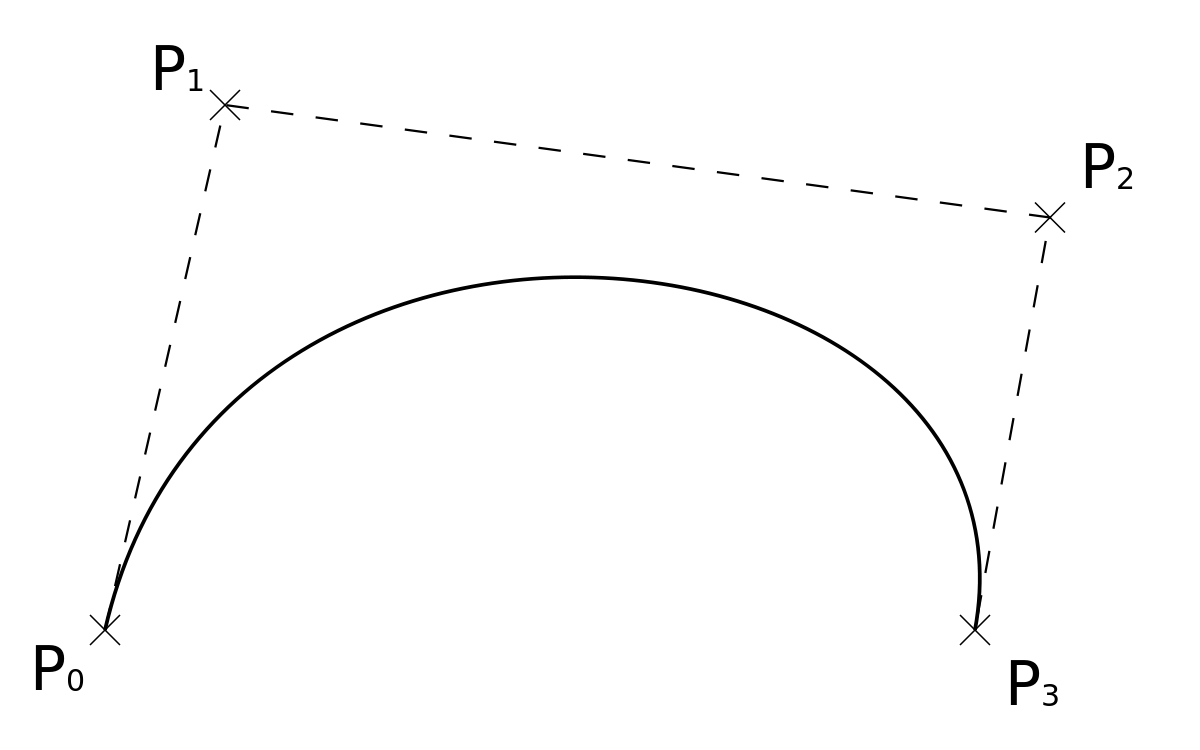
\includegraphics[width=0.66\textwidth]{otoczkawypukla.png}
\caption{Otoczka wypukła punktów $P_0, P_1, P_2, P_3$ (linie przerywane)}
\label{otoczkawypukla}
\end{figure}

\subsection{Kombinacja barycentryczna punktów}
Niech $W_0, W_1, \ldots, W_n$ będą punktami na płaszczyźnie, a $\alpha_0, \alpha_1, \ldots, \alpha_n$ liczbami rzeczywistymi takimi, że $\alpha_0 + \alpha_1 + \ldots + \alpha_n = 1$. Wtedy wyrażenie
$$ \alpha_0W_0 + \alpha_1W_1 + \ldots + \alpha_n W_n$$
nazywamy kombinacją barycentryczną punktów (jest ona zawsze określona jednoznacznie) i utożsamiamy z punktem postaci
$$\underbrace{W_0}_{\text{punkt}} + \underbrace{\alpha_1(W_1-W_0)+\alpha_2(W_2-W_0)+\ldots+\alpha_n(W_n-W_0)}_{\text{wektor}}$$

\subsection{Krzywa Beziera}
Dla danych punktów kontrolnych $W_0, W_1, \ldots, W_n$ na płaszczyźnie definiujemy krzywą Beziera stopnia $n$ jako
$$ P_n(t) := \sum\limits_{k=0}^{n}W_kB_k^n(t) \text{ dla } t\in[0,1]$$
\noindent Dla danego $t\in[0,1]$, $P_n(t)$ jest punktem na płaszczyźnie, mamy więc do czynienia z kombinacją barymetryczną punktów, co więcej punkt $P_n(t)$ należy do otoczki wypukłej $conv\{W_0, W_1, \ldots, W_n\}$. Oprócz tych własności mamy następujące:
\begin{itemize}
\item $P_n(0) = W_0, \ P_n(1)=W_n$
\item $P_n^{'}(0) = n(W_1-W_0)$
\item $P_n^{'}(1) = n(W_n-W_{n-1})$ 
\end{itemize}

\subsection{Wyznaczanie punktu $P_n(t)$ - algorytm de Casteljau}
Dla danego $t\in[0,1]$ wyznaczamy punkt $P_n(t)$ na krzywej Beziera za pomocą algorytmu de Casteljau:
\begin{itemize}
\item $W_k^{(0)} := W_0 \quad (0\leq k \leq n)$
\item $W_k^{(i)} := (1-t)W_k^{(i-1)}+tW_{k+1}^{(i-1)}\quad (i=0, 1, \ldots, n; \ k= 0, 1, \ldots, n-1)$
\end{itemize}
Wtedy punktem $P_n(t)$ jest $W_0^{(n)}$. Algorytm ten działa w czasie $O(n^2)$.

\begin{figure}[H]
\centering
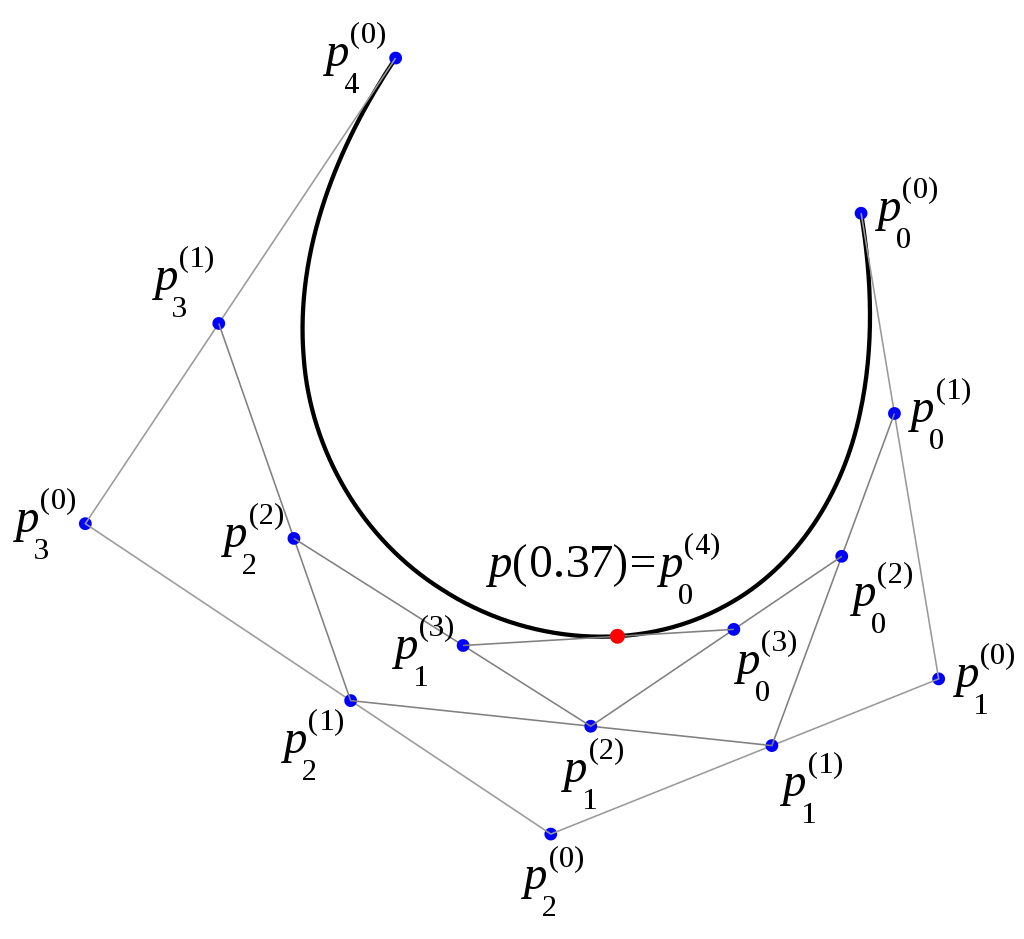
\includegraphics[width=0.66\textwidth]{decasteljau.png}
\caption{Interpretacja geometryczna algorytmu de Casteljau dla $t=0.37$}
\label{decasteljau}
\end{figure}



\newpage
\section{Aproksymacja średniokwadratowa na zbiorze dyskretnym}
Ideą aproksymacji jest jak najlepsze dopasowanie funkcji do chmury punktów, jednak rezygnujemy z interpolacji, aby zaoszczędzić pamięć.

\subsection{Norma średniokwadratowa na zbiorze dyskretnym}
Niech dane będą parami różne punkty $\mathcal{X}:=\{x_0, x_1, \ldots, x_N\}$ oraz funkcja $f$ określona na $\mathcal{X}$. Normę średniokwadratową funkcji $f$ na zbiorze $\mathcal{X}$ oznaczamy symbolem $||f||_2$ i definiujemy wzorem
$$ ||f||_2 := \sqrt{\sum\limits_{k=0}^{N} \left( f(x_k) \right)^{2}} $$
Norma średniokwadratowa to funkcjonał $||\cdot||_2: \mathcal{F}\to \mathbb{R}$, gdzie $\mathcal{F}$ jest zbiorem funkcji. Własnościami normy są (dla funkcji $f, g$):
\begin{itemize}
\item $||f||_2 = 0 \Leftrightarrow f(x_k)$ dla $k=0,1,\ldots, N$
\item $||\alpha\cdot f||_2 = |\alpha| \cdot ||f||_2$ dla $\alpha \in \mathbb{R}$
\item $||f+g||_2 \leq ||f||_2 + ||g||_2$ (nierówność trójkąta)
\end{itemize}

\noindent Aby sprawdzić czy dwie funkcje są do siebie podobne, należy obliczyć wartość wyrażenia
$$ ||f-g||_2 := \sqrt{\sum\limits_{k=0}^{N} \left( f(x_k)-g(x_k) \right)^{2}} $$
i na jej podstawie ocenić "bliskość" - jeśli otrzymany wynik jest mały, to $f, g$ są bliskie siebie.

\subsection{Znajdowanie elementu optymalnego funkcji $f$}
Dla danego zbioru $\mathcal{X}$ oraz funkcji $f$ określonej na $\mathcal{X}$ element $w^*\in\mathcal{F}$ nazywamy elementem optymalnym w sensie aproksymacji średniokwadratowej, że 
$$ ||f-w^*||_2 = \min\limits_{w\in\mathcal{F}}^{} ||f-w||_2  = \min\limits_{w\in\mathcal{F}}^{} \sqrt{\sum\limits_{k=0}^{N} \left( \underbrace{f(x_k)}_{y_k}-w(x_k) \right)^{2}} $$

\noindent Jeżeli aproksymacja średniokwadratowa napotka "odstające" obserwacje, tzn. niepasujące do reszty punktów z chmury, zostaną one praktycznie pominięte - współczynnik zwykle zmienia się bardzo minimalnie.\\
W sytuacji ogólnej wybieramy pewne funkcje podstawowe $g_0(x), \ldots, g_m(x)$ (np. $g_i(x)=x^i$, wtedy $lin\{g_0, \ldots, g_m\} \equiv \Pi_m$) i za model przyjmujemy $\mathcal{F} := \{ a_0g_0(x)+a_1g_1(x)+\ldots+a_mg_m(x): \ a_0, \ldots, a_m \in \mathbb{R}  \}$. Dla pomiarów $(x_k, y_k), \ (0\leq k \leq N)$ szukamy elementu optymalnego $w^*\in\mathcal{F}$ o własności:
$$ ||f-w^*||_2 = \min\limits_{w\in\mathcal{F}}^{} ||f-w||_2  = \min\limits_{a_0, \ldots, a_m \in \mathbb{R}}^{} \sqrt{E(a_0, \ldots, a_m)}$$
gdzie $E$ jest funkcją błędu zadaną przez 
$$E(a_0, \ldots, a_m) = \sum\limits_{k=0}^{N} \left( y_k - \underbrace{\sum\limits_{i=0}^{m} a_ig_i(x_k)}_{w(x_k)}  \right)^2 $$
Następnie szukamy minimum funkcji błędu $E$ za pomocą pochodnych cząstkowych (przyrównujemy je do zera), definiuje ono element optymalny $w^*$ w sensie aproksymacji średniokwadratowej na zbiorze dyskretnym.

\subsection{Wielomianowa aproksymacja średniokwadratowa na zbiorze dyskretnym}
Dla danego zbioru $\mathcal{X}$, funkcji $f$ na nim określonej i liczby naturalnej $m$ chcemy znaleźć wielomian $w_m^*\in\Pi_m$, dla którego
$$  ||f-w_m^*||_2 = \min\limits_{w_m\in\Pi_m}^{} ||f-w_m||_2 \equiv \min\limits_{w_m\in\Pi_m}^{} \sqrt{\sum\limits_{k=0}^{N} \left( y_k - w_m(x_n) \right)^{2}}$$
Efektywna metoda (o złożoności $O(mN)$) konstrukcji wielomianu optymalnego $w_m\in\Pi_m$ wymaga znajomości niżej opisanych narzędzi.

\subsubsection{Dyskretny iloczyn skalarny na zbiorze $\mathcal{X}$}
Dla funkcji $f,g$ iloczyn skalarny wyraża się wzorem
$$ (f,g)_N = \sum\limits_{k=0}^{N} f(x_k)g(x_k)$$

\subsubsection{Ortogonalność funkcji}
Funkcje $f$ oraz $g$ są ortogonalne gdy dla ustalonego iloczynu skalarnego zachodzi
$$ (f,g)_N = \sum\limits_{k=0}^{N} f(x_k)g(x_k) = 0$$

\noindent Układ funkcji $f_0, f_1, \ldots, f_m$ dla $m \leq N$ jest ortogonalny względem iloczynu skalarnego $(\cdot, \cdot)_N$ wtedy i tylko wtedy, gdy:
\begin{itemize}
\item $(f_i, f_j)_N = 0$ dla $i \neq j, \ 0 \leq i, j \leq m$
\item $(f_i, f_i)_N \textgreater 0$
\end{itemize}

\subsubsection{Ortogonalizacja Grama-Schmidta}
Dla danego układu liniowo niezależnych funkcji $g_0, g_1, \ldots, g_m$ oraz ustalonego wcześniej iloczynu skalarnego, układ funkcji $f_0, f_1, \ldots, f_m$ zadanych w następujący sposób rekurencyjny:
\begin{itemize}
\item $f_0 := g_0$
\item $f_k := g_k - \sum\limits_{j=0}^{k-1} \left( \frac{(g_k, f_j)_N}{(f_j, f_j)_N} \cdot f_j  \right) $ dla $k=1,2,\ldots, m$
\end{itemize}

\noindent jest układem ortogonalnym względem wybranego iloczynu skalarnego. \\
Aby znaleźć układ ortogonalny wielomianów generujących przestrzeń $\Pi_m$ możemy użyć ortogonalizacji Grama-Schmidta dla układu $1, x, x^2, \ldots, x^m$. Skonstruujemy go używając przedstawionej wyżej zależności rekurencyjnej dla $g_k(x) := x^k$ oraz $P_k \equiv f_k$ o własnościach:
\begin{itemize}
\item $P_k \in \Pi_k \setminus \Pi_{k-1}$ dla $k=0,1,\ldots, m; \ \Pi_{-1} = \emptyset$
\item $(P_k, P_l)_N = 0$ dla $k \neq l, \ 0 \leq k, l \leq m$
\item $(P_k, P_k)N \textgreater 0$
\end{itemize}

\noindent Ta metoda jednak jest zbyt droga, jej złożoność to $O(m^2N)$, a sama numeryczna realizacja ortogonalizacji Grama-Schmidta sprawia problemy numeryczne.

\subsubsection{Ciąg wielomianów ortogonalnych}
Z powodów przedstawionych w poprzednim paragrafie, skonstruujemy bazę przestrzeni $\Pi_m$ wykorzystując wielomiany $P_0, P_1, \ldots, P_m, \ (m \leq N)$ spełniające zależność rekurencyjną:
\begin{itemize}
\item $P_0(x)\equiv 1$
\item $P_1(x) = x - c_1$
\item $P_k(x) = (x-c_k)P_{k-1}(x)-d_kP_{k-2}(x) \quad (k = 2,3,\ldots, m; \ m \leq N)$
\end{itemize}
\noindent gdzie 
\begin{itemize}
\item $c_k := \frac{(xP_{k-1}, P_{k-1})_N}{(P_{k-1}, P_{k-1})_N} \text{ dla } ( 1 \leq k \leq m)$
\item $d_k := \frac{(P_{k-1}, P_{k-1})_N}{(P_{k-2}, P_{k-2})_N} \text{ dla } (2 \leq k \leq m)$
\end{itemize}
\noindent Zapis $(xP_{k-1}, P_{k-1})_N$ z licznika $c_k$ oznacza $\sum\limits_{k=0}^{N} x_kP_{k-1}(x_k)\cdot P_{k-1}(x_k)$. \\
Dzięki temu uzyskujemy koszt $O(mN)$, a numerycznie metoda działa bardzo dobrze.

\subsubsection{Rozwiązanie zadania} 
Wielomian optymalny $w_m^* \in \Pi_m$ wyraża się wzorem
$$ w_m^*(x) = \sum\limits_{k=0}^{m} a_kP_k(x), \quad a_k := \frac{(f,P_k)_N}{(P_k, P_k)_N}$$
\noindent gdzie $P_0, P_1, \ldots, P_m$ to ciąg wielomianów ortogonalnych względem dyskretnego iloczynu skalarnego dla zbioru $\mathcal{X}=\{ x_0, x_1, \ldots, x_N\}$. \\
Błąd wielomianowej aproksymacji średniokwadratowej wyraża się wzorem
$$ ||f-w_m^*||_2 = \sqrt{||f||_2 - \sum\limits_{k=0}^{m} \frac{(f,P_k)_N^2}{(P_k, P_k)_N}} $$

\noindent Możemy zaobserować, że $w_{m+1}^*(x) = w_m^*(x) + a_{m+1}P_{m+1}(x)$, czyli w łatwy sposób możemy budować ciąg wielomianów optymalnych, przy czym dla każdego kolejnego $m$ kontrolujemy wartość błędu. Wielomian $w_N(x)$ jest wielomianem interpolacyjnym dla danych $(x_k, y_k)$. \\
Aproksymacji tej warto używać dla $m \ll N$, jako że wtedy bardzo mocno kompresujemy dane.


\clearpage
\section{Kwadratury - całkowanie numeryczne}
Idea kwadratur czyli całkowania numerycznego polega na zastąpieniu trudnej funkcji $f(x)$ dla $x\in[a,b]$ poprzez inną, łatwiejszą - np. wielomian $w(x)$, jako że potrafimy je łatwo całkować, co pozwoli nam na przybliżenie $f(x)$.\\
$$w(x) \approx f(x) \text{ dla } x\in[a,b] \Rightarrow \underbrace{\int\limits_{a}^{b} f(x)dx}_{\text{trudna całka}} \approx \underbrace{\int\limits_{a}^{b} w(x)dx}_{\text{łatwa całka}}$$

\subsection{Funkcja podcałkowa, funkcja pierwotna}
Niech $f: \mathbb{R}\to\mathbb{R}$ będzie dowolną funkcją podcałkową dla $x \in [a,b]$. Funkcją pierwotną $F$ będzie wtedy funkcja spełniająca równanie
$$ F'(x) = f(x)$$
\noindent Wtedy możemy również obliczyć całkę oznaczoną korzystając z własności
$$\int\limits_{a}^{b} f(x)dx = F(b) - F(a)$$

\subsection{Metody obliczania całek}
\subsubsection{Całkowanie przez części}
Jeżeli funkcje $f, g$ są ciągłe oraz mają ciągłe pochodne, to
$$ \int f(x)g'(x)dx = f(x)\cdot g(x) - \int f'(x)\cdot g(x) dx$$

\subsubsection{Całkowanie przez podstawianie}
Jeżeli funkcję $f$ można zapisać w postaci $f(x)=g(h(x))\cdot h'(x)$, gdzie funkcja $h(x)$ ma ciągłą pochodną, to możemy skorzystać z całkowania przez podstawianie:
$$ \int f(x)dx = \int g(h(x))\cdot h'(x) dx = \underbrace{\left| \substack{t = h(x) \\ dt = h'(x)dx} \right|}_{\text{podstawienie}} = \int g(t)dt$$

\subsection{Kwadratura liniowa}
Dla danych parami różnych węzłów kwadratury $x_0^{(n)}, x_1^{(n)}, \ldots, x_n^{(n)}$ oraz liczb $A_0^{(n)}, A_1^{(n)}, \ldots, A_n^{(n)}$, kwadraturą liniową funkcji $f$ nazywamy wyrażenie postaci
$$ Q_n(f) := \sum\limits_{k=0}^{n}  A_k^{(n)} f(x_k^{(n)})$$
\noindent Naszym celem jest dobranie takich współczynników $A_k^{(n)}$ oraz węzłów $x_k^{(n)}$ kwadratury $Q_n$ w taki sposób, aby
$$ Q_n(f) \approx \int\limits_{a}^{b} f(x)dx = I(f)$$
\noindent dla $f$ należącej do "dużej" rodziny funkcji, tzn. współczynniki i węzły mają być uniwersalne (dobre dla wielu funkcji).

\subsubsection{Błąd kwadratury liniowej}
Błędem kwadratury liniowej $Q_n$ nazywamy
$$ R_n(f) := I(f) - Q_n(f) $$
\noindent Jeśli $R_n(f) =0$, to $I(f) = Q_n(f)$, a więc dokładnie całkujemy funkcję $f$.

\subsubsection{Rząd kwadratury liniowej}
Rząd kwadratury liniowej $Q_n$ wynosi $r$, jeśli:
\begin{itemize}
\item $\forall w \in \Pi_{r-1}\ \  I(w)=Q_n(w)$ (błąd kwadratury $R_n(w)=0$)
\item $\exists w \in \Pi_r \setminus \Pi_{r-1}\ \  I(w) \neq Q_n(w)$ (błąd kwadratury $R_n(w) \neq 0$)
\end{itemize}
\textbf{Twierdzenie:} Rząd kwadratury liniowej $Q_n$ jest nie przekracza $2n+2$.

\subsubsection{Strategia konstrukcji kwadratur}
Węzły $x_k^{(n)}$ oraz współczynniki $A_k^{(n)}$ dobieramy tak, aby rząd kwadratury liniowej $Q_n$ był jak największy. Oznacza to, że chcemy dokładnie całkować wielomiany tak wysokiego stopnia, jak to tylko możliwe.

\subsection{Kwadratura interpolacyjna}
Ideą kwadratury interpolacyjnej jest całkowanie wielomianu $L_n(x)$ zamiast funkcji $f(x)$ w węzłach $x_0^{(n)}, x_1^{(n)}, \ldots, x_n^{(n)}$. Wielomian $L_n \in \Pi_n$ musi spełniać warunek $L_n(x_k^{(n)}) = f(x_k^{(n)})$ dla $k=0,1,\ldots, n$ i jest on postaci
$$ L_n(x) = \sum\limits_{k=0}^{n} \lambda_k(x)f\left( x_k^{(n)} \right) \text{, gdzie } \lambda_k(x) = \prod\limits_{\substack{i=0 \\ i \neq k}}^{n} \frac{x-x_i}{x_k-x_i} \in \Pi_n$$
\noindent Scałkujmy postać Lagrange'a wielomianu interpolacyjnego:
$$ \int\limits_{a}^{b} L_n(x)dx = \int\limits_{a}^{b} \left[ \sum\limits_{k=0}^{n} \lambda_k(x) f\left( x_k^{(n)} \right) \right] dx = \sum\limits_{k=0}^{n} \left[ \int\limits_{a}^{b} \lambda_k(x)dx \cdot f\left( x_k^{(n)} \right) \right] = Q_n(f)$$
\noindent W takiej postaci kwadratura interpolacyjna jest przedstawiona takim wzorem jak wcześniej. Jej współczynniki mają postać
$$ A_k^{(n)} := \int\limits_{a}^{b} \left( \lambda_k(x) \right) = \int\limits_{a}^{b} \left(  \prod\limits_{\substack{i=0 \\ i \neq k}}^{n} \frac{x-x_i^{(n)}}{x_k^{(n)}-x_i^{(n)}} \right)$$
\noindent \textbf{Twierdzenie:} Kwadratura liniowa $Q_n$ ma rząd większy lub równy $n+1$ wtedy i tylko wtedy, gdy jest ona kwadraturą interpolacyjną.

\subsection{Kwadratura Newtona-Cotesa}
Ideą tej kwadratury jest stworzenie kwadratury interpolacyjnych dla węzłów równoodległych, a więc przyjmujemy, że są nimi 
$$x_k^{(n)}=a+\underbrace{\frac{b-a}{n}}_{h} \cdot k$$
\noindent Kwadratura Newtona-Cotesa będzie wtedy zdefiniowana przez
$$ Q_n^{NC}(f) := \sum\limits_{k=0}^{n} A_k^{(n)} f(a+hk) $$

\subsubsection{Współczynniki kwadratury Newtona-Cotesa}
Jawnym wzorem na współczynniki kwadratury Newtona-Cotesa jest
$$ A_k^{(n)} = \frac{(-1)^{n-k}h}{k!(n-k)!} \int\limits_{0}^{n} \left[ \prod\limits_{\substack{j=0 \\ j \neq k}}^{n} (t-j) \right] dt$$
\noindent gdzie $t$ jest taką zmienną, że $x=a+th$.

\subsubsection{Błąd kwadratury Newtona-Cotesa}
$$ R_n(f) = 
\begin{cases}
\frac{f^{(n+1)}(\eta)}{(n+1)!} \int\limits_{a}^{b} p_{n+1}(x)dx		& (n=1,3,5,\ldots) \\
\frac{f^{(n+2)}(\alpha)}{(n+2)!} \int\limits_{a}^{b} x p_{n+1}(x)dx	& (n=2,4,6,\ldots)
\end{cases}
$$
\noindent dla $p_{n+1}(x) = \left( x-x_0^{(n)} \right)\left( x-x_1^{(n)}\right)\ldots\left( x-x_n^{(n)}\right)$.

\subsubsection{Rząd kwadratury Newtona-Cotesa}
Rząd kwadratury Newtona-Cotesa wynosi $n+1$ dla $n$ nieparzystych oraz $n+2$ dla $n$ parzystych. Warto jednak pamiętać, że pod względem rzędu, kwadratury Newtona-Cotesa są słabym narzędziem, bo jesteśmy "na granicy" danego oszacowania dla rzędu kwadratur interpolacyjnych.

\subsection{Wzór trapezów, złożony wzór trapezów}
Wzór trapezów jest jednym ze wzorów do przybliżonego obliczania całek oznaczonych. Dla danej funkcji $f$ na przedziale $x\in[a,b]$ możemy oszacować wartość całki $\int\limits_{a}^{b}f(x)dx$ za pomocą kwadratury
$$ Q_1(f) := \frac{b-a}{2} \left( f(a)+f(b) \right) $$

\begin{figure}[H]
\centering
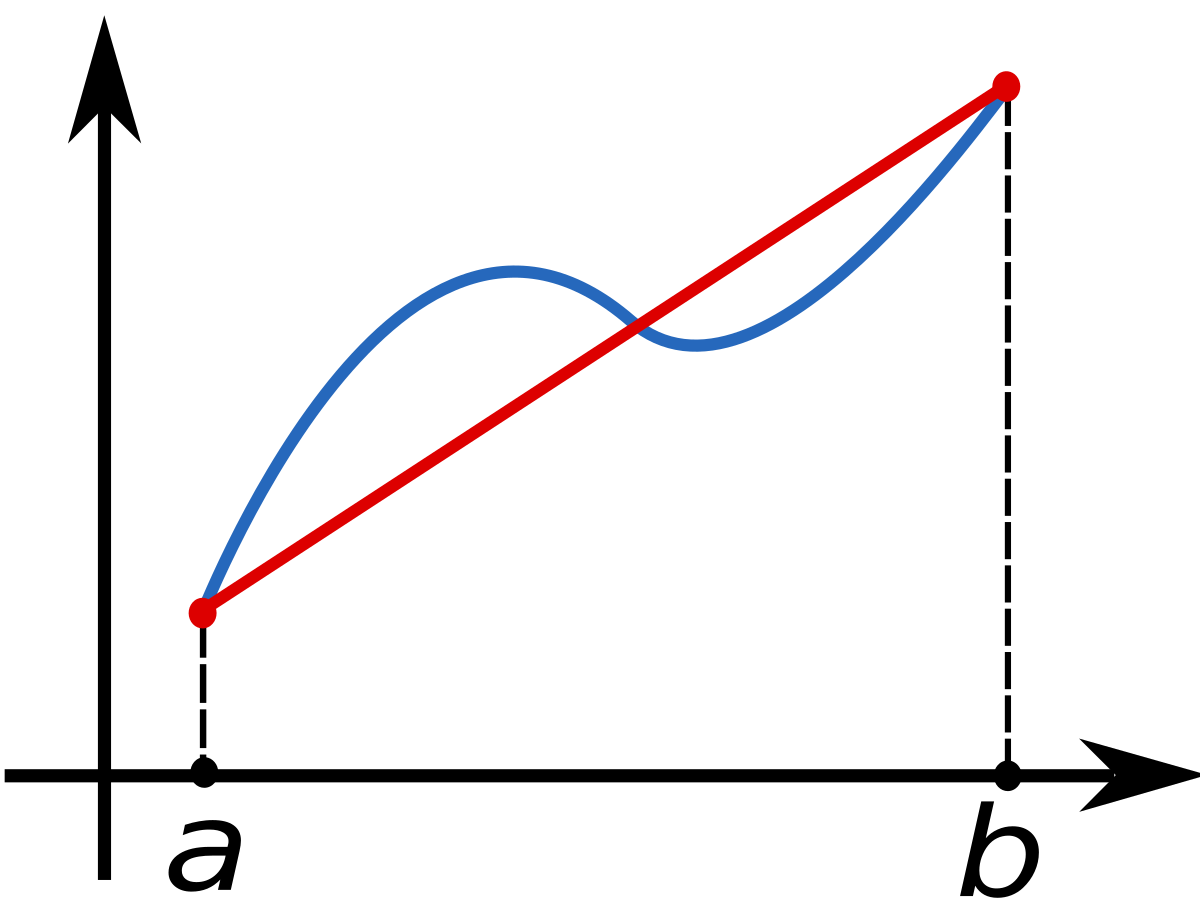
\includegraphics[width=0.5\textwidth]{wzortrapezow.png}
\caption{Zasada działania wzoru trapezów}
\label{wzortrapezow}
\end{figure}

\noindent Rząd tej metody wynosi $2$. Jednokrotne wykorzystanie wzoru trapezów może dokładnie obliczyć całkę (w każdym przypadku) tylko z funkcji liniowej i stałej, dlatego powinniśmy używać \textbf{złożonego wzoru trapezów}, tzn. przedział $[a,b]$ dzielimy na równe części i na każdej z nich stosujemy wzór trapezów. Otrzymujemy wtedy dla węzłów $t_k := a+h_nk$, $(k=0,1,\ldots, n)$, $h_n:=\frac{b-a}{n}$ wzór
$$ \int\limits_{a}^{b} f(x)dx = T_n(f) + R_n^T $$
\noindent gdzie $T_n(f)$ jest złożonym wzorem trapezów, a $ R_n^T$ błędem złożonego wzoru trapezów. Złożony wzór trapezów wyraża się wzorem
$$ T_n(f) := h_n \sum\limits_{k=0}^{n}{}^{''} f(t_k) = h_n(\frac{1}{2}f(t_0) + f(t_1) + \ldots + f(t_{n-1}) + \frac{1}{2}f(t_n)$$
\noindent \textbf{Oznaczenie:} $\sum{}^{''}x$ - pierwszy i ostatni wyraz mnożony jest przez $\frac{1}{2}$. \\
\textbf{Twierdzenie:} Jeśli funkcja $f\in C^2[a,b]$, to 
$$R_n^T(f):= \frac{a-b}{12}h_n^2 f''(\eta_n)$$
\noindent dla $\eta_n \in (a,b)$, a $h_n^2$ jest rzędu $O(n^{-2})$.\\
\noindent \textbf{Twierdzenie:} Jeśli $f\in C[a,b]$, to $\lim\limits_{n\to\infty} T_n(f)=\int\limits_{a}^{b} f(x)dx$.

\subsection{Wzór Simpsona, złożony wzór Simpsona}
Wzór Simpsona jest kolejnym sposobem przybliżonego obliczania całek oznaczonych. Polega on na interpolacji kwadratowej w trzech punktach: $a, \ \frac{a+b}{2}, \ b$. Kwadratura ta wyznaczona jest wzorem
$$ Q_2(f) := \frac{b-a}{2} \left( \frac{1}{3} f(a) + \frac{4}{3} f \left( \frac{a+b}{2} \right) +  \frac{1}{3} f(b) \right) $$

\begin{figure}[H]
\centering
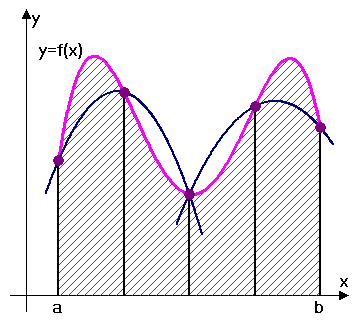
\includegraphics[width=0.35\textwidth]{wzorsimpsona.png}
\caption{Zasada działania złożonego wzoru Simpsona dla $4$ części}
\label{wzorsimpsona}
\end{figure}

\noindent Rząd tej metody wynosi $4$, a więc możemy dokładnie obliczyć całki nawet trzeciego stopnia. Jednak tutaj podobnie jak w przypadku wzoru trapezów, warto byłoby skorzystać z podziału przedziału na parzystą liczbę równych podprzedziałów i dla każdych trzech kolejnych punktów stosować wzór Simpsona, aby dokładniej wyliczać całki oznaczone. Otrzymujemy wtedy dla węzłów $t_k := a+h_nk$, $(k=0,1,\ldots, n)$, $h_n:=\frac{b-a}{n}$ wzór
$$ \int\limits_{a}^{b} f(x)dx = S_n(f) + R_n^S $$
\noindent gdzie $S_n(f)$ jest złożonym wzorem Simpsona, a $ R_n^S$ błędem złożonego wzoru Simpsona. Złożony wzór Simpsona wyraża się wzorem
$$ S_n(f) := \frac{h_n}{3} \left( 2\sum\limits_{k=0}^{m}{}^{''} f(t_{2k}) + 4\sum\limits_{k=1}^{m} f(t_{2k-1}) \right)$$
\noindent \textbf{Twierdzenie:} Jeśli $f\in C^4[a,b]$, to
$$ R_n^S(f) := \frac{a-b}{180} h_n^4 f^{(4)}(\alpha_n)$$
\noindent dla $\alpha_n \in (a,b)$, a $h_n^4$ jest rzędu $O(n^{-4})$.\\
\noindent \textbf{Twierdzenie:} Jeśli $f\in C[a,b]$, to $\lim\limits_{n\to\infty} S_n(f) = \int\limits_{a}^{b} f(x)dx$. \\
\noindent \textbf{Obserwacja:} $\underset{(n=2m)}{S_n(f)} = \frac{4T_n(f) - T_m(f)}{4-1}$ - ekstrapolacja

\subsection{Metoda Romberga}
Niech $n=2^k$ dla $k \in \mathbb{N}$, $h_k := \frac{b-a}{2^k}$, $x_i^{(k)} := a+ih_k$ dla $i=0,1,\ldots, 2^k$. Zdefiniujmy $T_{0,k} := T_{2^k}(f) = h_k\sum\limits_{i=0}^{2^k}{}^{''}f(x_i^{(k)})$ (złożone wzory trapezów). Kolejne elementy $T_{m,k}$ dla $k = 0,1,\ldots$ oraz $m=1,2,\ldots$ definiujemy rekurencyjnie za pomocą wzoru
$$ T_{m, k} := \frac{4^mT_{m-1, k+1} - T_{m-1, k}}{4^m-1} $$

\subsubsection{Tablica Romberga}
Tworzenie tablicy Romberga przebiega w sposób pokazany na przykładzie poniżej (podobnie jak w ilorazach różnicowych).
$$
\begin{array}{ccccccc} % każde "c" odpowiada za wyśrodkowanie kolumny, także liczba c = liczba kolumn
T_{0,0}	\\	
T_{0,1}	&	T_{1,0}	\\
T_{0,2}	&	T_{1,1}	&	T_{2,0}	\\
T_{0,3}	&	T_{1,2}	&	T_{2,1}	&	T_{3,0}	\\
T_{0,4}	&	T_{1,3}	&	T_{2,2}	&	T_{3,1}	&	T_{4,0}	\\
\vdots 	&	\vdots 	&	\vdots 	&	\vdots 	&	\vdots 	&	\ddots 	\\
T_{0,m}	&	T_{1, m-1}	&	T_{2, m-2}	&	\ldots 		&	\ldots 		& 	\ldots 		& 	T_{m, 0}
\end{array}
$$
\noindent Przeważnie każda kolejna kolumna tablicy Romberga zbiega szybciej do wartości całki, a najszybsza zbieżność występuje na przekątnej tablicy.\\
\textbf{Twierdzenie:} $\lim\limits_{k\to\infty} T_{mk} = \int\limits_{a}^{b} f(x)dx$ dla ustalonego $m$ i funkcji ciągłej $f$.\\
\textbf{Twierdzenie:} $\lim\limits_{m\to\infty} T_{mk} = \int\limits_{a}^{b} f(x)dx$ dla ustalonego $k$ i funkcji ciągłej $f$.

\subsubsection{Efektywne obliczanie wartości w pierwszej kolumnie}
Wartość funkcji $f$ możemy obliczyć tylko raz w każdym punkcie i ją zapamiętać, jako że dla każdego kolejnego $k$ (przy $n=2^k$) będziemy dzielić przedział na coraz mniejsze równe części. Dzięki temu w pierwszym kroku obliczymy $f(0)$ oraz $f(1)$i, w kolejnym $f(\frac{1}{2})$, w kolejnym $f(\frac{1}{4})$ oraz $f(\frac{3}{4})$ itd.
\begin{figure}[H]
\centering
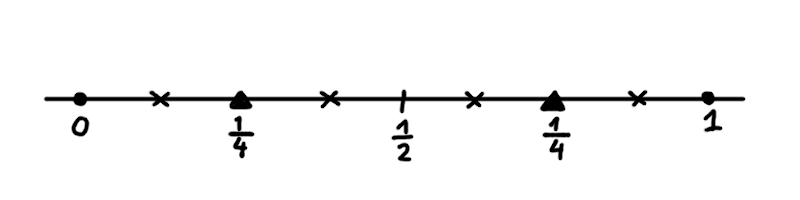
\includegraphics[width=0.85\textwidth]{romberg.png}
\caption{Przykład efektywnego obliczania $T_{0,n}$ na przedziale $[0,1]$}
\label{romberg}
\end{figure}

\subsection{Kwadratura Gaussa}
Kwadraturami Gaussa nazywamy kwadratury $Q_n$ rzędu $2n+2$. Są one zawsze interpolujące, jako że ich rząd jest większy od $n+1$. Współczynniki wyrażone są wzorem
$$ A_k^{(n)} = \int\limits_{a}^{b} \left[ \prod\limits_{\substack{i=0 \\ i \neq k}}^{n} \frac{x-x_i^{(n)}}{x_k^{(n)}-x_i^{(n)}} \right] dx$$
\noindent Przyjmijmy $a=-1, \ b=1$, tzn. weźmy całki $\int\limits_{-1}^{1}f(x)dx$ - wtedy będziemy mówić o \textbf{kwadraturach Gaussa-Legandre'a}. Należy jeszcze znaleźć węzły, które można obliczyć poprzez znalezienie miejsc zerowych w wielomianach Legandre'a wyrażone rekurencyjnym wzorem:
\begin{itemize}
\item $P_0(x) \equiv 1$
\item $P_1(x) \equiv x$
\item $P_k(x) = \frac{2k-1}{k}xP_{k-1}(x)-\frac{k-1}{2}P_{k-2}(x)$ dla $k=2,3,\ldots$
\end{itemize}
Miejsca zerowe wielomianu $P_{n+1}$ są węzłami kwadratury Gaussa-Legandre'a mającej rząd równy $2n+2$. Nie ma jawnego wzoru na obliczanie ich, jednak ich wartości można przybliżyć numerycznie (chociażby używając metody bisekcji, stycznych czy siecznych). Współczynniki i węzły są od dawna dokładnie stablicowane, więc możemy ich używać w łatwy sposób.


\clearpage
\section{Algorytmy numeryczne algebry liniowej}

\subsection{Krótkie przypomnienie z algebry (macierze)}
Macierzą $A$ nazywamy tablicę elementów rozmiaru $n \times m$, której elementami $a_{ij}$ są liczby rzeczywiste. Standardowymi zapisami macierzy są
$$
A = \left[
\begin{array}{cccc}
a_{11}	& 	a_{12}	& 	\ldots 		& a_{1m} \\
a_{21}	& 	a_{22}	& 	\ldots 		& a_{2m} \\
\vdots 	& 	\vdots		& 	\ddots		& \vdots \\
a_{n1}	& 	a_{n2}	& 	\ldots 		& a_{nm} 
\end{array}
\right] \in \mathbb{R}^{n\times m} \text{ oraz } A = \left[ a_{ij} \right] \in \mathbb{R}^{n\times m}
$$
\noindent gdzie $n$ jest liczbą wierszy, a $m$ liczbą kolumn. Dla $n=m$ mówimy o macierzy kwadratowej o stopniu $n$.

\subsubsection{Podstawowe działania na macierzach}
Niech $A = \left[ a_{ij} \right] \in \mathbb{R}^{n\times m}$, $B = \left[ b_{ij} \right] \in \mathbb{R}^{n\times m}$, $C = \left[ c_{ij} \right] \in \mathbb{R}^{m\times k}$. Podstawowymi działaniami na macierzach są:
\begin{itemize}
\item dodawanie/odejmowanie: $A \pm B =: D = \left[ d_{ij} \right] \in \mathbb{R}^{n\times m}$, $d_{ij} = a_{ij} \pm b_{ij}$
\item mnożenie przez skalar: $A \cdot \alpha =: E = \left[ e_{ij} \right] \in \mathbb{R}^{n\times m}$, $e_{ij} = a_{ij} \cdot \alpha$ $(\alpha \in \mathbb{R})$
\item mnożenie macierzy: $A \cdot C =: F = \left[ f_{ij} \right] \in \mathbb{R}^{n\times k}$, $f_{ij} := \sum\limits_{h=1}^{m} a_{ih}\cdot c_{hj}$
\item transpozycja ${}^T$: $A^T =  \left[ a_{ji} \right] \in \mathbb{R}^{m \times n}$
\end{itemize}

\subsubsection{Wyznacznik macierzy kwadratowej}
Wyznacznikiem macierzy nazywamy jednoznacznie określoną funkcję $det: \mathbb{R}^{n\times n} \to \mathbb{R}$. Przyporządkowuje ona macierzy pewną liczbę rzeczywistą. Istnieje jawny wzór na obliczanie wyznacznika, jednak jego złożoność czasowa to $O(n!)$. Bardziej opłacalną metodą jest zastosowanie przekształceń elementarnych do zamiany macierzy na macierz trójkątną:
$$
A = \left[
\begin{array}{cccc}
a_{11}	& 	0		& 	\ldots 		& 0 \\
a_{21}	& 	a_{22}	& 	\ddots		& \vdots \\
\vdots 	& 	\vdots		& 	\ddots		& 0 \\
a_{n1}	& 	a_{n2}	& 	\ldots 		& a_{nn} 
\end{array}
\right]
$$
\noindent Wtedy wyznacznik można łatwo obliczyć ze wzoru:
$$ det(A) = a_{11} \cdot a_{22} \cdot \ldots \cdot a_{nn} $$
\noindent Podstawowymi własnościam wyznaczników są:
\begin{itemize}
\item $det(A) = det(A^T)$
\item $det(A\cdot B) = det(A) \cdot det(B)$
\end{itemize}

\subsubsection{Odwracanie macierzy kwadratowej}
Zdefiniujmy macierz jednostkową $I_n \in \mathbb{R}^{n\times n}$ w następujący sposób:
$$
I_n = \left[
\begin{array}{cccc}
1		& 	0		& 	\ldots 		& 0 \\
0		& 	1		& 	\ddots		& \vdots \\
\vdots 	& 	\ddots	 	& 	\ddots		& 0 \\
0		& 	\ldots		& 	0 		& 1 
\end{array}
\right]
$$
\noindent Macierzą odwrotną do $A \in \mathbb{R}^{n\times n}$ nazywamy taką macierz $A^{-1} \in \mathbb{R}^{n\times n}$, że spełniona jest zależność
$$  A^{-1} \cdot A = A \cdot A^{-1} = I_n$$
\noindent Macierz odwrotna do $A$ istnieje wtedy i tylko wtedy, gdy $det(A)\neq 0$.

\subsubsection{Układ równań liniowych}
Weźmy układ równań liniowych następującej postaci:
$$
\begin{cases}
a_{11}x_{1}+a_{12}x_{2}+\dots+a_{1n}x_{n}= b_1 \\
a_{21}x_{1}+a_{22}x_{2}+\dots+a_{2n}x_{n}= b_2 \\
\ \ \ \vdots \\
a_{n1}x_{1}+a_{n2}x_{2}+\dots+a_{nn}x_{n}= b_n
\end{cases}
\equiv A\cdot x = b
$$
\noindent gdzie $A=\left[ a_{ij} \right] \in \mathbb{R}^{n\times n}$ oraz $b = \left[ \substack{b_1 \\ \vdots \\ b_n} \right]$ są danymi, a $x = \left[ \substack{x_1 \\ \vdots \\ x_n} \right]$ szukanymi niewiadomymi. Taki układ ma jednoznaczne rozwiązanie wtedy i tylko wtedy, gdy $det(A)\neq 0$. Rozwiązaniem takiego układu równań liniowych jest:
\begin{align*}
Ax &= b  /\cdot_{L} A^{-1} \\
A^{-1}(Ax) &= A^{-1}b \\
\underbrace{A^{-1}A}_{I_n}x &= A^{-1}b \\
x &= A^{-1}b
\end{align*}

\subsubsection{Wzory Cramera}
Mając macierz $A$, wektor $b$ oraz $x$ możemy utworzyć macierz $A_k$ poprzez zamianę $k$-tej kolumnty macierzy $A$ na elementy wektora $b$. Wtedy kolejnymi wartościami wektora $x$ będą wyrazy
$$ x_k = \frac{det(A_k)}{det(A)}$$ 

\subsubsection{Przykład rozwiązania układu równań liniowych}
Niech 
$A= \left[ \begin{array}{cc} 1 & 0.99 \\ 0.99 & 0.98 \end{array} \right]$, $b = \left[ \begin{array}{c} 1.99 \\ 1.97 \end{array} \right]$, 
$\widetilde{b} = b +  \left[ \begin{array}{c} -0.000097 \\ +0.000106 \end{array} \right] = \left[ \begin{array}{c} 1.989903\\ 1.970106 \end{array} \right]$, a więc $b \approx \widetilde{b}$. Rozwiązując układ $Ax=b$ otrzymamy $x = \left[ \begin{array}{c} 1 \\ 1 \end{array} \right]$, jednak dla układu $Ax=\widetilde{b}$ otrzymamy $x = \left[ \begin{array}{c} 3.0000 \\ -1.0203 \end{array} \right]$. Możemy stąd wywnioskować, że zadanie jest źle uwarunkowane i należy być ostrożnym nawet dla prostych danych.

\subsection{Rozwiązywanie układów równań o macierzy trójkątnej dolnej}
$$
\left\{
\begin{array}{llll}
l_{11}x_{1}  &= b_1 \\
l_{21}x_{1}+l_{22}x_{2} &= b_2 \\
\ \ \ \vdots & \ \ \ \   \vdots \\
l_{n1}x_{1}+l_{n2}x_{2}+\dots+l_{nn}x_{n} &= b_n
\end{array}
\right.
\equiv Lx=b
$$
\noindent gdzie $L$ jest macierzą trójkątną dolną (tzn. wszystkie pozostałe wartości są $0$), $b$ wektorem znanych wartości, a $x$ wektorem niewiadomych. Taki układ możemy rozwiązać w czasie $O(n^2)$ za pomocą poniższej metody:
$$ x_k = \frac{b_k - \sum\limits_{j=1}^{k-1} l_{kj}x_j}{l_{kk}} $$
\noindent dla $k = 1, \ldots, n$, $l_{kk} \neq 0$. W podobny sposób możemy rozwiązać układ trójkątny górny, jednak w tym przypadku wartości $x$ liczymy od $x_n$ do $x_1$.

\subsection{Metoda faktoryzacji rozwiązywania układów równań liniowych}
Załóżmy, że układ $Ax=b$ ma jednoznaczne rozwiązanie ($A\in \mathbb{R}^{n\times n}$ oraz $x, b \in \mathbb{R}^n$) i że znamy taką macierz trójkątną dolną $L \in \mathbb{R}^{n\times n}$ oraz macierz trójkątną górną $U \in \mathbb{R}^{n\times n}$, że $A = L\cdot U$. Możemy wtedy pokazać, że rozwiązaniem wyjściowego układu jest rozwiązanie dwóch układów trójkątnych.
\begin{align*}
Ax &= b \\
LUx &= b \\
L \underbrace{(Ux)}_{y} &= b
\end{align*}
\noindent Przyjmijmy, że $y:=Ux$, wtedy $Ly=b$ (układ trójkątny). Stąd w łatwy sposób możemy wyznaczyć najpierw $y$, a następnie rozwiązać drugi układ równań postaci $Ux=y$, którego rozwiązaniem jest szukany $x$, będący rozwiązaniem wyjściowego układu
$$
Ax=b \Leftrightarrow
\begin{cases}
Ly = b \text{, gdzie znamy } L \text{ oraz } b \\
Ux = y \text{, gdzie znamy } U \text{ oraz } y \text{ z powyższego równania}
\end{cases}
$$
\noindent Rozwiązanie takiego układu zajmuje czas $O(n^2)$, jednak musimy znać rozkład $LU$ macierzy, który nie zawsze istnieje.

\subsection{Rozkład trójkątny macierzy $\equiv$ rozkład LU}
Weźmy macierz $A = \left[ a_{ij} \right] \in \mathbb{R}^{n\times n}$ taką, że wyznacznik wszystkich jej minorów głównych jest różny od zera, tzn.
$$ 
det
\left[
\begin{array}{cccc}
a_{11} &  a_{12} & \ldots &  a_{1k} \\	
a_{21} &  a_{22} & \ldots &  a_{2k} \\	
\vdots  &   \vdots & \ddots &  \vdots \\	
a_{k1} &  a_{k2} &  \ldots &  a_{kk} \\	
\end{array}
\right]
\neq 0 \text{ dla } k = 1, 2, \ldots, n
$$
\noindent Wówczas istnieje dokładnie jedna para macierzy $L, U  \in \mathbb{R}^{n\times n}$, gdzie $L$ jest macierzą trójkątną dolną \textbf{z jedynkami na przekątnej}, a $U$ jest macierzą trójkątną górną, spełniającą równość $A=L\cdot U$. Jawnym wzorem na rozkład $LU$ o złożoności czasowej $O(n^3)$ jest
$$
\begin{cases}
u_{ij} = a_{ij} - \sum\limits_{k=1}^{i-1} l_{ik}u_{kj} \text{ dla } (i \leq j) \\
l_{ij} = \frac{1}{u_{jj}}\cdot \left( a_{ij} - \sum\limits_{k=1}^{j-1} l_{ik}u_{kj}\right) \text{ dla } (i \textgreater  j)
\end{cases}
$$
\noindent Dzięki rozkładowi $LU$ i wiedzy o postaci wyznacznika macierzy trójkątnej możemy łatwo obliczyć wyznacznik ze wzoru:
$$ det(A) = det(L\cdot U) = det(L) \cdot det(U) = \underbrace{l_{11}\cdot \ldots \cdot l_{nn}}_{1\text{ (przekątna)}} \cdot u_{11}\cdot \ldots \cdot u_{nn} = \prod\limits_{i=1}^{n} u_{ii}$$
\noindent czy odwrócić macierz ($det(A)\neq 0$):
$$ A=LU \Leftrightarrow A^{-1} = (LU)^{-1} = U^{-1} \cdot L^{-1}$$
\noindent Odwrotnością macierzy trójkątnej jest zawsze macierz trójkątna tego samego typu.

















\end{document}